\documentclass[11pt]{article}
\usepackage[margin=1.05in]{geometry}
\usepackage{graphicx,booktabs,amsmath,amssymb,microtype,xcolor}
\usepackage[labelfont=bf,font=small]{caption}
\usepackage{tikz}
\usetikzlibrary{arrows.meta,positioning,fit,backgrounds}
\usepackage[hidelinks]{hyperref}

\definecolor{sblue}{HTML}{2a78d6}
\definecolor{sorange}{HTML}{eb6834}
\definecolor{saqua}{HTML}{1baf7a}
\definecolor{sgrid}{HTML}{d9d8d4}
\newcommand{\code}[1]{\texttt{\small #1}}

\title{\bf One Symbolic Interaction Protocol,\\ and What Fits Inside It}
\author{Jacob Valdez\thanks{Built with Claude Opus 5 in Claude Code; every
commit records the collaboration. Code, data and the full result files:
\url{https://github.com/JacobFV/symbolic-ai-001}.}}
\date{August 2026}

\begin{document}
\maketitle

\begin{abstract}
\noindent
We define a single interaction protocol---an agent consumes symbolic
observations, emits symbolic actions, and receives a reward and a next
observation---and ask how much of machine learning fits inside it without
distorting the tasks. We show, as an executable check rather than an argument,
that language-model pretraining is the special case in which the action is a
predictive distribution and the reward is $\log p(x_{t+1}\mid x_{\le t})$: on
trained checkpoints and held-out text, the return accumulated through
\code{Environment.step} and the log-likelihood computed by ordinary batched
cross-entropy agree to $|\Delta| = 1.9\times10^{-5}$ over 512 token positions.
Inside this protocol we compare a 13.97M-parameter transformer against
\emph{non-neural} learners---no gradients, no learned tensors, tens of discrete
parameters, CPU only. A 26-parameter induced world model, fitted in 0.14\,s,
solves a gridworld $16\times$ larger than any it was fitted on at 1.00 success
where the transformer scores 0.00; a parameter-free program synthesizer scores
1.00 on rule families held out of training where a neural specialist scores
exactly 0.00. We then build a 180-lesson procedurally generated language
curriculum (179 admissible under a floor-and-determinism test) and use it as a
measuring instrument: it reveals that symbolic induction is \emph{bimodal}
(exact where the capability lies inside its hypothesis space, at chance where it
does not) while the neural arm is \emph{uniformly mediocre} (above chance on
$10/14$ pilot lessons, master of none). The resulting capability map turns ``what
should we build next'' into a measurement. We then close the loop: an unattended
agent, guarded against the two ways such a loop can cheat, reads the map and
builds the mechanism it names. We report the negative results---gradients
still win decisively at natural-language modelling, 82 of 106 capabilities remain
at chance---and two measurement bugs that the instrument caught in our own work.
\end{abstract}

\section{Introduction}

The agent--environment loop is old, and the claim that everything is an instance
of it is cheap. What is not cheap is the glue: supervised learning ships a
dataloader, reinforcement learning a \code{gym.Env}, LLM agents a
rollout-and-rubric API, computer use a container protocol. Any claim about ``one
agent across everything'' is therefore mostly a claim about integration code.

We take the glue seriously and put all of it at one boundary. Above the boundary
there is exactly one contract; below it, every substrate keeps its own reset
semantics, rewards, graders and canonical metrics. The contribution is not the
formalism but what the formalism then lets us measure:

\begin{enumerate}\itemsep2pt
\item that next-token pretraining is literally a special case, checked
      numerically on trained models (\S\ref{sec:equiv});
\item a like-for-like comparison of neural and non-neural learners inside one
      protocol, where the non-neural side wins decisively on extrapolation and
      loses decisively on language modelling (\S\ref{sec:gen});
\item a 180-lesson procedurally generated curriculum with an admission test, used
      as an instrument rather than a benchmark (\S\ref{sec:curriculum});
\item a capability map that selects the next mechanism to build by measurement
      (\S\ref{sec:mechanisms}).
\end{enumerate}

\section{The protocol}

A \emph{symbol} is an immutable, hashable, typed node whose value may contain
other symbols, so one primitive covers tokens, numbers, identifiers, predicates,
relations, lists, AST nodes, graph references, records---and distributions over
symbols. That last case is what lets supervised prediction be an \emph{action}
rather than a separate mode of the framework.

\begin{align*}
\text{Environment:}\quad & \mathrm{reset}(\text{seed}) \to (O^*,\ \text{info})\\
                         & \mathrm{step}(A^*) \to (O^*, r, \text{term}, \text{trunc}, \text{info})\\
\text{Agent:}\quad & A : (S_{\text{agent}}, O^*) \to (S_{\text{agent}}, A^*)
\end{align*}

Agent state is passed in and returned rather than hidden in the object, which is
what makes agents forkable for search and replayable from a trajectory. Every
environment declares typed, inspectable observation and action \emph{spaces};
both discrete actions (\code{LEFT}) and structured ones
(\code{Call(function="search", args=\{\ldots\})}) are first class.

We borrowed deliberately: from Gymnasium, \code{reset(seed)} and the
\code{terminated}/\code{truncated} distinction; from Prime Intellect's
\code{verifiers}, dataset-backed episodes and graders that own their reward
semantics; from OpenEnv, an explicit \code{state()} view so a containerized
backend can implement the same protocol. We did not borrow any commitment to an
optimizer: the learner protocol is one method, \code{update(trajectories)}, and
no environment knows it exists.

\begin{figure}[t]
\centering
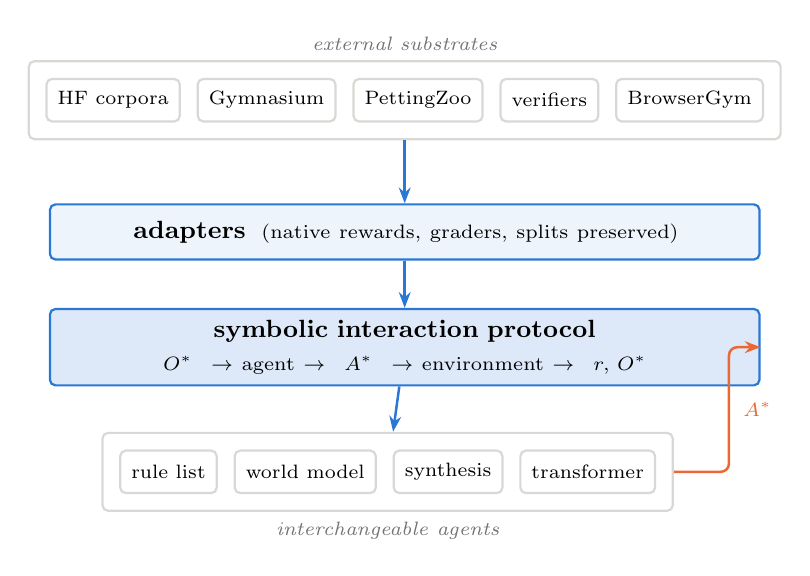
\begin{tikzpicture}[
  font=\small,
  box/.style={draw=sgrid,line width=0.8pt,rounded corners=2pt,align=center,
              inner sep=4pt,minimum height=7mm},
  sub/.style={box,fill=white,font=\scriptsize,minimum height=5.4mm},
  arr/.style={-{Stealth[length=2mm]},draw=sblue,line width=0.9pt}]

\node[sub] (a1) {HF corpora};
\node[sub,right=2mm of a1] (a2) {Gymnasium};
\node[sub,right=2mm of a2] (a3) {PettingZoo};
\node[sub,right=2mm of a3] (a4) {verifiers};
\node[sub,right=2mm of a4] (a5) {BrowserGym};
\node[draw=sgrid,line width=0.8pt,rounded corners=2pt,inner sep=6pt,
      fit=(a1)(a5),label={[font=\scriptsize\itshape,text=black!55]above:external substrates}] (subs) {};

\node[box,below=8mm of subs,fill=sblue!8,draw=sblue,text width=0.72\linewidth]
     (ad) {\textbf{adapters} \;\scriptsize(native rewards, graders, splits preserved)};
\node[box,below=6mm of ad,fill=sblue!16,draw=sblue,text width=0.72\linewidth]
     (proto) {\textbf{symbolic interaction protocol}\\[1pt]
       \scriptsize $O^* \rightarrow$ agent $\rightarrow A^* \rightarrow$ environment $\rightarrow r,\,O^*$};

\node[sub,below=8mm of proto,xshift=-30mm] (g1) {rule list};
\node[sub,right=2mm of g1] (g2) {world model};
\node[sub,right=2mm of g2] (g3) {synthesis};
\node[sub,right=2mm of g3] (g4) {transformer};
\node[draw=sgrid,line width=0.8pt,rounded corners=2pt,inner sep=6pt,
      fit=(g1)(g4),label={[font=\scriptsize\itshape,text=black!55]below:interchangeable agents}] (ags) {};

\draw[arr] (subs) -- (ad);
\draw[arr] (ad) -- (proto);
\draw[arr] (proto) -- (ags);
\draw[arr,draw=sorange,rounded corners=3pt]
      (ags.east) -- ++(7mm,0) |- node[pos=0.25,right=0.5mm,font=\scriptsize,text=sorange]{$A^*$}
      (proto.east);
\end{tikzpicture}
\caption{Uniformity lives at the adapter boundary, not inside the substrates.
Every environment keeps its native semantics; every agent sees only symbols.}
\label{fig:arch}
\end{figure}

\section{Prediction is interaction, checked}
\label{sec:equiv}

For a sequence $x_1\ldots x_n$, set $O^*_t = x_1\ldots x_t$, let $A^*_t$ be a
predictive distribution over the vocabulary, and let
$r_t = \log p(x_{t+1}\mid x_{\le t})$. The transition appends $x_{t+1}$ (teacher
forcing) or the agent's own argmax (free running).

The claim that this ``is'' language modelling is easy to assert and easy to get
subtly wrong, so we made it a test. At unit level, with a randomly initialized
transformer, the episode return equals the batched sum of $\log p$ over the same
positions to $2\times10^{-3}$; per step $\text{nll} = -r$ and
$\text{ppl}=e^{\text{nll}}$; and a uniform predictive policy earns exactly
$\log(1/V)$ per step, which is the calibration check that the reward really is a
log-probability. End-to-end, on trained checkpoints and held-out FineWeb-Edu
text restricted to identical positions:

\begin{center}\small
\begin{tabular}{lrrr}
\toprule
model & positions & $\sum\log p$ (loop) & $|\Delta|$ \\
\midrule
mixture-trained & 512 & $-2398.2746$ & $1.9\times10^{-5}$\\
LM-only         & 512 & $-2324.7483$ & $2.3\times10^{-4}$\\
\bottomrule
\end{tabular}
\end{center}

Two consequences. Maximum-likelihood pretraining is not a different objective
from RL-style credit assignment here; it is the case where every sample carries
weight 1 and the transition ignores the action. And the trainer may use batched
tensors for throughput without changing the objective, because this equality is
what licenses the shortcut.

\section{Two kinds of agent in one protocol}

\paragraph{The neural arm.} \emph{symbolic-ai-001} is a 13.97M-parameter
decoder-only transformer (6 layers, $d=384$, context 512, byte-level BPE over
FineWeb-Edu text \emph{plus} serialized symbolic structures). It is trained by
one loss over the action segment of a symbolic step,
$L = -\sum_i w_i \log p_\theta(a_i \mid o_i) / \sum_i w_i|a_i|$, where the choice
of $w$ selects the paradigm: $w=1$ on a token stream is next-token pretraining,
$w = \exp((G-b)/\beta)$ on episodes is advantage-weighted regression. It was
trained for 8{,}000 steps (16.0 min, one NVIDIA GB10) on a mixture of FineWeb-Edu,
SST-2, a gridworld, MiniGrid, three reasoning environments and tool calls.

\paragraph{The symbolic arms.} A learner qualifies as symbolic here if it uses no
gradients, no learned real-valued tensor, keeps all fitted structure discrete and
countable, prints as a program a person can read, and runs on a CPU. Six were
built; the two that matter most are \emph{world-model induction} (learn each
action's effects, preconditions and the world's bounds, plus what the environment
rewards, then plan inside the induced schema) and \emph{query-program induction}
(induce a program that computes the answer from the structure of the
observation).

What world-model induction learns from 21{,}394 gridworld transitions, in
\textbf{0.14\,s of CPU} and 26 discrete parameters, is exactly the world's laws:
\begin{quote}\ttfamily\scriptsize
RIGHT : move(+1,0) unless wall(+1,0) within [0,size)\\
PICKUP: add holds(agent,key); del at(key,0,0)\\
GOAL~~: at(goal,0,0) $\wedge$ holds(agent,key)
\end{quote}
The bound \code{[0,size)} is read from the observation, so the same operator is
correct at any scale---which is the mechanism behind
Figure~\ref{fig:scaling}.

\section{Generalization}
\label{sec:gen}

\begin{figure}[t]
\centering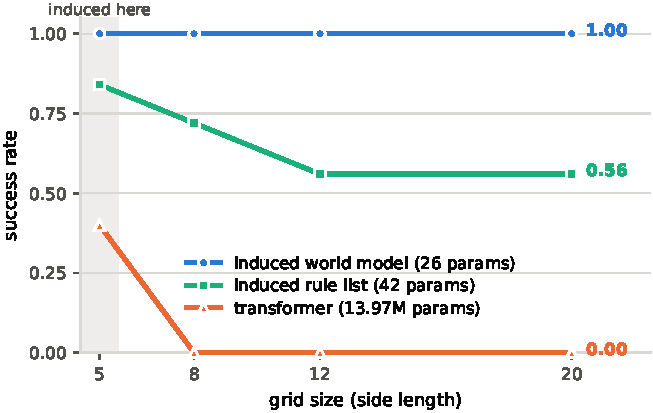
\includegraphics[width=0.94\linewidth]{figs/scaling.pdf}
\caption{Induced on $5\times5$ gridworlds with 3 walls, evaluated up to
$20\times20$ with 24 walls (25 held-out episodes per cell). The induced schema is
flat across a $16\times$ change in state-space size; the transformer is at zero
the moment the world stops looking like its training data.}
\label{fig:scaling}
\end{figure}

\paragraph{Scaling.} Figure~\ref{fig:scaling}. A non-learning planner given the
\emph{true} model but a bounded search budget degrades faster than the induced
one ($0.80 \to 0.00$ across the same range), so learning the schema does not
merely save data---it makes search tractable by abstracting it.

\paragraph{A goal nobody trained for.} The same 26 parameters, re-aimed at three
goals absent from training (\emph{hold the key}; \emph{stand on the goal square};
\emph{stand where the key is}), achieve $1.00$ each on the first attempt with no
new data. A policy---symbolic or neural---has no mechanism for this: it would
need fresh demonstrations per goal.

\paragraph{Held-out rule families.} A sequence environment generates from a hidden
rule. Five families appear in training; five structurally analogous ones appear
only at evaluation:

\begin{center}\small
\begin{tabular}{lrrr}
\toprule
agent & params & train fam. & held-out fam. \\
\midrule
program synthesizer & \bf 0 & \bf 1.000 & \bf 1.000 \\
neural specialist & 13{,}969{,}152 & 0.975 & \bf 0.000 \\
random & 0 & 0.025 & 0.000 \\
\bottomrule
\end{tabular}
\end{center}

\noindent The network reproduces its training families almost perfectly and
scores \emph{exactly zero} on families it has not seen. The synthesizer does not
distinguish the two cases, because it has no training distribution to be off.

\paragraph{Imported knowledge.} On SST-2, a 17-parameter rule list induced
\emph{on top of} an imported lexicon (12{,}065 terms, ${\sim}100$\,kB) reaches
0.765 in 0.7\,s of CPU, against 0.585 for the transformer. The ablation is the
point: induction alone reaches 0.480 and the prior alone 0.600. Importing
knowledge is not cheating if the system can still learn; it is refusing to spend
petaflops rediscovering a dictionary.

\paragraph{Where gradients win.} A counting-based variable-order model on the same
corpus and vocabulary reaches held-out perplexity 179.4 (order 5, 20M tokens,
199\,s CPU) against 51.9 for the transformer, and its memory grows with distinct
contexts rather than with a parameter budget---a 40M-token configuration
exhausted host memory. Natural-language modelling is a real loss for the symbolic
side, and no framing changes that.

\section{A curriculum as an instrument}
\label{sec:curriculum}

We implemented a 170-environment curriculum spanning symbol grounding to
open-world research, plus 14 pilot lessons: \textbf{180 lessons, 179 admissible},
one honestly marked \code{spec} because it is a loop rather than a question.
Lessons are \emph{procedural generators}, not datasets, so evaluation episodes are
new worlds and vocabularies rather than a held-out sample, and ground truth is
exact rather than annotated. Grammar and ontology travel in \code{info}, visible
to the evaluator and never to the agent.

A lesson counts only if it passes an admission test: exact ground truth, answer
in vocabulary, uniform guesser near chance, \emph{constant (majority) guesser
under threshold}, and determinism. Floors alone are far from sufficient. Most
generators were additionally audited by an independent oracle that re-derives
each answer from the observation alone, and by heuristic audits that simulate the
shortcut an unthinking agent would take. That found real defects: one lesson was
100\% solvable from distractor name suffixes; another fell to ``pick the
candidate with most variables'' at 0.61; a third yielded 0.47 to averaging
payoffs under the \emph{wrong} dimension---noise masquerading as signal.

\begin{figure}[t]
\centering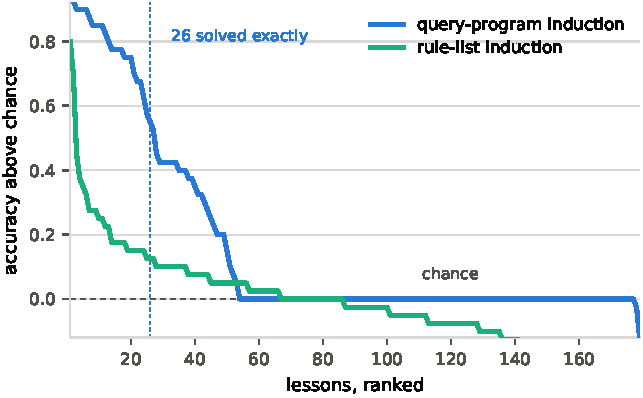
\includegraphics[width=0.94\linewidth]{figs/bimodality.pdf}
\caption{Per-lesson accuracy above chance, lessons ranked. Symbolic induction is
bimodal: exact where the capability lies inside its hypothesis space, at chance
where it does not. (The rule-list curve covers fewer lessons because it errors on
some.)}
\label{fig:bimodality}
\end{figure}

\paragraph{The shape, not the average.} On the 14-lesson pilot, query-program
induction solves $11/14$ at $\ge0.90$ while a transformer finetuned on the whole
curriculum solves \emph{0} and is above chance on $10/14$. Symbolic induction is
bimodal; the network is uniformly mediocre. A single ``language score'' would
hide exactly this. Figure~\ref{fig:bimodality} shows the same shape across all
179 lessons.

Profiling all 179 lessons across three arms costs \textbf{two minutes of CPU},
which is what makes the loop in \S\ref{sec:mechanisms} practical.

\section{The capability map selects the next mechanism}
\label{sec:mechanisms}

\begin{figure}[t]
\centering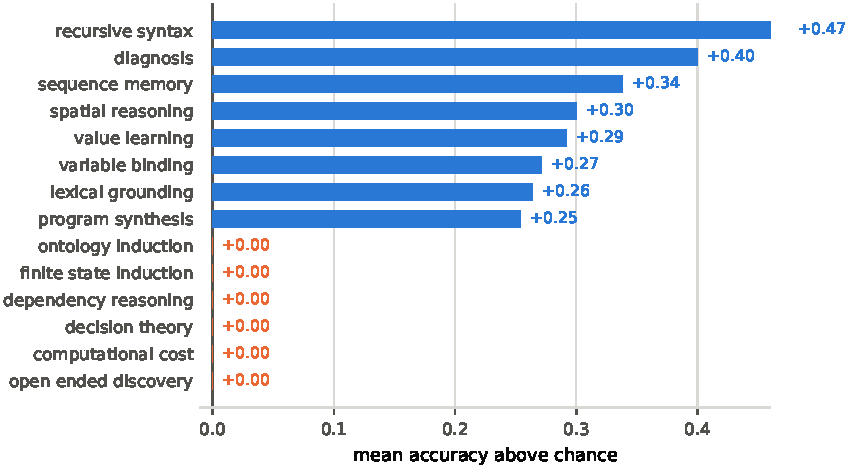
\includegraphics[width=0.94\linewidth]{figs/capabilities.pdf}
\caption{Mean accuracy above chance per declared capability (top eight and the
six most-represented at chance). 82 of 106 capabilities remain at chance.}
\label{fig:caps}
\end{figure}

Averaging each arm over the capabilities that lessons declare turns ``what should
we build?'' into a measurement (Figure~\ref{fig:caps}). The capabilities at
chance were not a list of hard problems but a list of \emph{absent mechanisms}.
We built them and re-measured (Figure~\ref{fig:mech}); each is a general
combinator whose parameters are induced, never a lesson-specific rule.

\begin{figure}[t]
\centering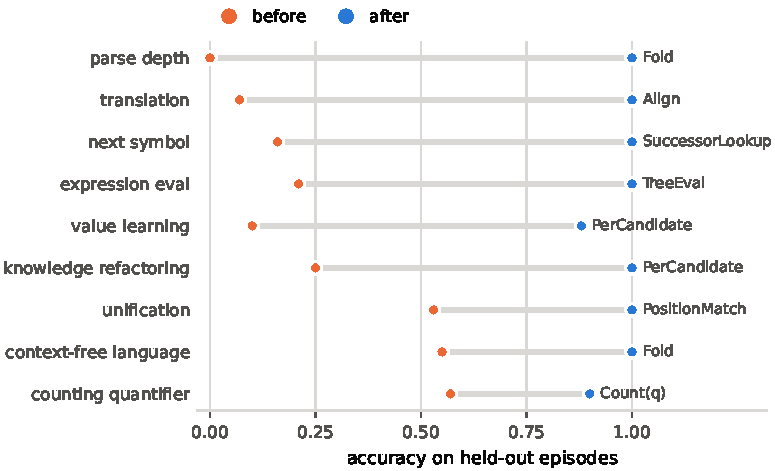
\includegraphics[width=0.94\linewidth]{figs/mechanisms.pdf}
\caption{Each mechanism and the lesson it unlocked, measured on held-out
episodes. Nine lessons moved; seven to exact.}
\label{fig:mech}
\end{figure}

Two episodes are worth reporting because they were informative rather than
incidental.

\emph{Alignment failed three times.} Positional zip fails because the translation
lesson permutes word order; order-free co-occurrence intersection fails because
the correspondence is underdetermined by co-occurrence; what works is searching
the small space of reorderings and keeping those whose induced lexicon is
consistent across every sentence pair. ``Alignment between symbol systems'' is
therefore not one mechanism: it decomposes into lexical correspondence and
structural reordering, which must be induced \emph{jointly} because neither is
identifiable alone.

\emph{A fitted mechanism made things worse.} Adding a tree evaluator---which
induces what each operator symbol \emph{means} by fitting the assignment that
reproduces the answers---lifted expression evaluation from 0.21 to 1.00 but
regressed three other lessons. Most programs here are enumerated, so scoring them
on the episodes used to choose them is honest; a program that fits parameters can
beat a better unfitted one on the very episodes it was fitted to. Selecting on a
held-out slice fixed it, at no cost to the enumerated programs.

\section{Closing the loop}
\label{sec:loop}

If the capability map names the next mechanism and a full re-measurement costs two
minutes, the iteration can be automated. We ran an unattended agent that reads the
deficit briefing, builds one general mechanism, and re-measures---with the
verification held \emph{outside} its control, because a loop optimising ``lessons
solved'' has exactly two exploits: make the lessons easier, or weaken the
admission test. A cycle is merged only if the tests pass, the verified and
registered lesson counts hold, no lesson's chance floor moves, no arm's solved
count falls, and the diff touches no lesson file or admission code at all.

In its first hour the loop read the map, identified stateful sequential execution
as the largest gap, and built an abstract machine---store, sequencer, loop and
branch---whose opcode semantics are induced rather than given. Verified
independently before merging:

\begin{center}\small
\begin{tabular}{lrr}
\toprule
lesson & before & after\\
\midrule
procedural language     & 0.10 & \bf 1.00\\
interpreter learning    & 0.12 & \bf 1.00\\
compiler construction   & 0.30 & \bf 1.00\\
\midrule
solved / 179            & 23   & \bf 26\\
\bottomrule
\end{tabular}
\end{center}

\noindent Its own note on the interpreter lesson is the sort of thing we wanted
the loop to find: several opcode assignments reproduced every demonstration and
then disagreed on the held-out program, so five demonstrations did not identify
the hypothesis; requiring that two opcodes never mean the same thing made all
sixty episodes uniquely determined, and \emph{that constraint is itself an induced
parameter}. Few-shot fitting is not few-shot learning unless the examples
identify the hypothesis.

The guard also earned its place immediately, by rejecting a cycle that changed
nothing---which is how we discovered the reproducibility defect in
\S\ref{sec:negative}.

\section{Negative results and threats to validity}
\label{sec:negative}

We report these because a paper that reports only its wins is not measuring
anything.

\textbf{Gradients win at language.} Perplexity 179.4 versus 51.9, and the
counting model's memory is unbounded in a way a parameter budget is not.

\textbf{Most of the curriculum is unsolved.} 26 of 179 lessons at $\ge0.90$; the
large majority of declared capabilities remain at chance. The curriculum is far ahead of the learner, which we
consider the correct state for an instrument but which forecloses any claim of
general competence.

\textbf{Reactive policies cannot explore.} A 5-parameter induced MiniGrid policy
scores 1.00 at $5\times5$ and 0.00 at $8\times8$, because the goal leaves the
egocentric view. One discrete knob (randomize when no rule fires) restores 0.96.
At $16\times16$ the goal is never visible at reset and no memoryless policy can
succeed---an architecture limit, not a scale limit, and the neural arm fails
identically.

\textbf{Data requirements invert.} The first world model never learned that walls
block movement, because the expert teacher avoids walls. Adding 400 random
episodes took it from $0.60/0.30/0.25$ to $1.00/1.00/1.00$. Policy learners want
expert data; model learners want diverse data. Separately, no amount of expert
data reveals that \code{PICKUP} requires a key---a competent teacher never tries
it---so that precondition had to come from the representation (STRIPS delete-lists
are preconditions) rather than from data.

\textbf{Two measurement bugs in our own work.} The admission test condemned a
lesson on sampling noise: a constant guesser's score is itself a random variable,
and a balanced binary lesson trips a fixed threshold about one run in six.
Borderline cases are now re-measured at $4\times$. More seriously, program
induction was \emph{not reproducible across processes}: facts live in a
\code{frozenset}, so hash randomization changed enumeration order, which decided
ties, so borderline lessons flipped between runs and every earlier number carried
unacknowledged flap. This was caught by the guard on an automated cycle that
changed nothing and was still rejected. Sorted iteration and a tie-break on
program text fixed it; two full sweeps in separate processes now agree exactly.

\textbf{Scope.} Single seeds per cell; differences under $\approx0.1$ on 25--50
episodes are not resolvable. Energy was never measured in joules---the GPU was
shared with an unrelated job throughout---so the efficiency claim is stated in
time and parameters ($\approx10^4$ in fit time, $\approx10^6$ in parameters) and
not in watts. The curriculum's generators and one of its learners were written by
the same effort, which is a real threat to validity that only an external
benchmark can address.

\section{Related work}

The protocol borrows lifecycle ideas from Gymnasium, from Prime Intellect's
\code{verifiers} (the taskset, harness and runtime separation; graders that own their
semantics), and from OpenEnv. The symbolic learners are recognisable classics:
separate-and-conquer rule induction, STRIPS action-model learning, enumerative
program synthesis with observational-equivalence pruning, variable-order Markov
modelling. Our contribution is not any single algorithm but placing them and a
transformer behind one contract so the comparison is like-for-like, and building
an instrument sharp enough to say where each one ends. The closest contemporary
motivation is the observation that per-task program induction, rather than
amortization into weights, is what solves ARC-style tasks.

\section{Conclusion}

Inside a single symbolic interaction protocol, next-token pretraining is a
special case that can be verified numerically; non-neural learners with tens of
discrete parameters beat a 13.97M-parameter transformer decisively on
extrapolation, novel goals and unseen rule families, at $10^{-4}$ of the fitting
cost; and gradients remain decisively better at modelling natural language. The
useful artefact is less any of these results than the instrument: a 180-lesson
generator suite with an admission test, cheap enough to run in two minutes, whose
capability map names the next mechanism to build. Following that map---by hand, and then by an unattended agent that built a
working abstract machine on its first cycle---produced eight new capabilities in
a day, and caught two bugs in our own measurements along the way.

\small
\paragraph{Reproduction.}
\begin{quote}\ttfamily\scriptsize
python -m symbolic.experiments.curriculum\_full\\
python -m symbolic.experiments.symbolic\_suite\\
pytest tests/ conftest.py -q
\end{quote}

\end{document}
